% Chapter 6

\chapter{Experiment Two - Business Transactional Data} % Main chapter title

\label{Chapter6} % For referencing the chapter elsewhere, use \ref{Chapter1} 

\lhead{Chapter 6. \emph{Experiment Two - Business Transactional Data}} % This is for the header on each page - perhaps a shortened title

%----------------------------------------------------------------------------------------

\section{Introduction}

In the previous chapter, an experiment was undertaken with a large UK geographic postcode data set through the proposed visualisation model. In this chapter, business transactional data set will be analysed through the proposed visualisation model with more complex and even diverse than the previous experiment data set. The data set holds business transactional data from a commercial company for over seven years of trading. This data ranges from sales data to customer feedback, and also includes web based business analytical information. It has been processed by the proposed information visualisation model in order to find any hidden trends within the data, and to explore the analytics for the business, in order to allow for more effective resource utilisation in a real time business environment. The second part of the experiment also have a bespoke tool developed under the same visualisation model for non-enterprise data sets. The two parts are supported by various figures extracted from a live system. 

\section{Acquisition and Data Analysis}

The acquisition and data analysis elements of the information visualisation model are discussed in this section. A transaction can mean different things depending on the context, but in this particular instance a transaction is defined as a sequence of information exchange and related work (such as database updating) that is treated as a unit for the purposes of satisfying a request\cite{williamson1979transaction}. Transactional data can cover finances, logistics or work related data, involve anything from a purchase order and shipping status to employee work hours and insurance costs and claims. Once it has been processed, transactional data is then grouped with its associated master and reference data to create the transactional records. A relevant date and time are added to this, along with the relevant reference data needed for each particular transaction record. Most studies conducted resulting in research and working papers use synthetic data sets in order to produce their control group \cite{axelsson2000generation}. This is normally done using random number generators to help create more data on the fly, and is usually adequate for research conditions into new data analysis techniques \cite{council2005transaction}.

In the first part of this experiment, these large data sets were made available directly to the visualisation system for purely business and data analysis purposes. The data sets which have been obtained for the first part of the experiment consist of several million records, collected from various sections of the existing enterprise systems. The data consists of various different factors and user behaviours, including:

\begin{itemize}
\item Geographical Location
\item IP Address
\item Transaction amount
\item Transactional type
\item Shopping Times
\item Sales Transactions   
\item Staff Behaviour
\item Conversion Figures 
\end{itemize}

The details along with resources such as drivers and vehicle information for transport companies were provided in huge masses of raw data sets for analytical purposes. The proposed information visualisation model process involves various different data analysis techniques, followed by representation (or visualising the data), couples with the interactive layers in the visualisation model. The term enterprise 2.0 within an organisation is used, it is usually referring to an environment of the business where data is available in a normalised form and accessed through web services and APIs. The enterprise environment is a very modern idea, and has been designed with a multi-user and multi-developer base in mind. It's because of this new, modern idea that the data analysis can be processed in a real time environment but before diving into full data analysis in an enterprise environment, the applications are highlighted below. Like any other modern application, an enterprise application has to be reliable, perform well, provide intuitive and effective user interface and live up to high levels of data usage without struggling \cite{fowler2002patterns}. Enterprise application is typically characterised by these three attributes:

\begin{itemize}
\item 	Multi-component Enterprise:  Where applications are rarely utilised for smaller amounts of data. When it is developed into a multi-user, multi-developer machine, it becomes a sophisticated multi-component application that can handle and manipulate massive amount of data while using streams of built in extensive parallel processing, resources distributed by various networks and very complex logic with ease. Such applications can be deployed across multiple platforms and inter-operate with a variety of different other applications, and it is an incredibly long lived solutions. Accounting, enterprise assets management and database management system are some examples of multi-component applications.

\item	Business Oriented: The specific purpose of enterprise applications is to meet very specific business requirements. The application encodes business policies, processes, rules and entities, and is developed within the business organisation to suit their needs. The application is then deployed in a variety of manners, all of which are responsive to the business needs. Reporting, resource management, business performance and business intelligence are some examples of such applications.

\item	Mission Critical: For a lot of businesses, enterprise applications fulfil a mission critical role. For this reason, an enterprise application must be able to stand up to a lot of pressure, and robust enough to endure constant operations. It must also be flexible to allow for extreme scalability and instant deployment while being accessible enough to allow for effective maintenance, monitoring and administration. Critical infrastructure and crisis management are a couple of areas where mission critical applications are utilised.

\end{itemize}

The combination of these qualities understandably makes the task of developing an enterprise application an incredibly daunting and challenging. This made even more difficult by the new trend towards businesses making rapidly increasing demands of their applications. This is supported by the rapid improvement of computer hardware and software within the business world, combined with a quickening global economic competition. This competition and the opportunities it spawns, have created a unique environment in which business systems are forced to respond at faster and faster speed in order to deliver unparallelled levels of performance and service. As these demands continue to rise, the developers of the applications are pushed to automate more and more of their business applications, to build their software even faster - enabling it to serve more and more users and process a rapidly growing mass of data. Putting all of these challenges aside, the sheer power, complexity and rapid change of technology used in the building of these corporate solutions make simple and efficient development of applications even more difficult.

The process of designing and developing an enterprise application is a complex one, and in order understand the process, some of the requirements are listed below.

\begin{itemize}
\item 	The business goals.
\item	How soon the application must be delivered.
\item	It's budget.
\item	How many people will develop, test and maintain the application.
\item	How many concurrent users the application will need to support.
\item	The importance of performance in the application and the ease of use.
\item	The hardware it needs to run on.
\item	Where it will be deployed.
\item	What security is required for this business.
\item	How long the application will be used for.
\end{itemize}

To understand relationship between such complex and conflicting requirements that requires a systematic approach. It needs to simplify the model and reduce the levels of complexity in order to provide an organised way to design and build applications, and ones that chart the optimum course among the many requirements of the applications. That process is demonstrated in Figure 3.3. At the root of any visualisation process lies in data analysis. Using the proposed methodology, the system will be able to establish what environment the visualisation request originated in - an Enterprise 2.0 environment or a non-enterprise environment. The origin determination will decide how the request is processed. If the request originated in an enterprise environment then the proposed system will already be aware of the data structure, and will have direct access to the data sets through web services and API's. 

The mashup application will also be able to understand the data structure, and therefore will be able to directly access information as and when it is needed for the visualisation process. This system will have direct and multiple connections with data sources in real time as the data sources change and alter. The proposed system application will be updated and new data acquired from the source, as shown in Figure 3.3. The benefits of processing data in a familiar environment is that the first four main stages of data analysis (acquire, parse, filter and mine) can all be achieved through basic API's and web services or web intelligent agents(PHP functions). For example, if a particular application requires sales figures for it's visualisation, a mashup system combined with web intelligent agents could search for and access the sales figures through API's in the familiar XML format before passing it on to the system as another layer for the visualisation process. Any information the system required could be easily and directly accessed, and that's the key benefit and essential for any system to work within a known environment.

Data acquisition is a process is executed through web intelligent agents and the instructions for this usually come from a business supportive model. This model is designed by management within the business, and is used to initiate and process certain tasks. These tasks are made up of clear instructions to the system, including what information needs to be identified and fetched for analysis. The visualisation model describes the rationale and process of how the business will create, deliver and captures value within an economic, social, cultural or other context. The process of constructing a business model is an essential part of the business strategy. and within the model there is a business process or method, comprised of a collection of related and structured activities, all of which produce specific services or products to serve a particular goal for customers. This often easily visualised as a flow chart, with a sequence of activities with interwoven decision points, or when using a process matrix, a sequence of activities with relevant rules all based on data within this process. There are generally three types of business processes, all of which are detailed below \cite{van2003business}.

\begin{itemize}
\item 	Management processes: These are the processes that govern the operation of a specific system. A typical management process includes corporate governance and strategic management.

\item	Operational processes: These are processes that constitute the core business model and help create the primary value stream within the business offering. For example, taking orders from customers, or opening a bank account within a branch are both operational procedures.

\item	Supporting processes: These supporting processes support the core processes within the business. Examples of this include the accounting and human resource management.
\end{itemize}

Every business process starts with a mission and ends with the achievement of that business objective. A process oriented business can break down the barriers of structural departments, and do their best to avoid any functional silos. A business process can be easily separated into several different sub-processes, each of which has its own attributes and properties. They also contribute their individual talents to achieving the collective goal, or super-process. To analyse the business processes of an organisation would typically start with mapping out the processes and sub-processes right down to the activity level \cite{aguilar2004business}. The parsing of data is not required in this case - as the information is already in a known structure within the business. As an example, the database table is illustrated in Figure 6.1. The data for this table has been acquired from an enterprise environment where the data about bookings is stored. There are approximately 74 attributes in the table, equating to 74 columns within a spreadsheet format. Each of the 74 attributes represent different information about different bookings. The data set contains millions of records of various business attributes. For example, customers, bookings, resource, staff and assets information are available in the data set.\\

\begin{figure}[H]
\centering
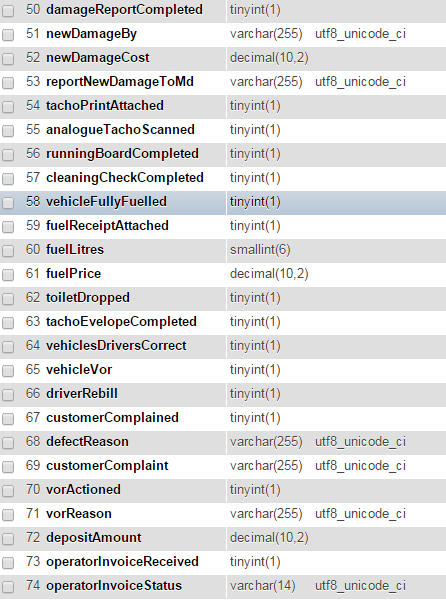
\includegraphics[scale=0.8]{chapter6/booking_table_3}
\caption{Booking Table from Database Overview}
\end{figure}

In this situation, the refining and filtration stages of data analysis are not required, as the business support models know exactly which fields within the data sets need to be retrieved for analysis purposes. The database table shown in Figure 6.1 helps to clarify the nature of the attributes. The system has the ability to transfer data into simple visual content. For example, if the system is asked a question (or query initiated) by the manager through a business supportive model (in this case, how much fuel does a booking cost?), an analysis model will read that command and will only retrieve information which is related to the fuel from that database. In this instance, the system will fetch the attribute 61 as shown in Figure 6.1 labelled as Fuel Price. The visualisation model will then be able to use and process that information, and turn it into a visualisation output to allow the decision makers to see and understand it easily. The process is simple in an enterprise environment, in a non-enterprise environment it needs to be handled differently. If the data sets are not accessible through traditional means such as API's, or if it is in an unknown structure, the mashup application must then request mining tasks. The acquisition and data analysis process for non-enterprise data is handled through a separate and dedicated information visualisation tool created on the same principle of the proposed information visualisation model called Visualixer. The Visualixer then process raw data and remove, filter and then parse and mine information into the MySQL database. The data is then available to the data representation layer for visualising. The full system features of Visualixer are explained below, along with a brief summary of the more important sections and features.

\subsection{The Visualixer System for Non-enterprise Data Sets}

The Visualixer system has been specifically designed to deal with data that is in a non-enterprise origin. Usually data extracted from this kind of environment is taken from a complex system and this means that the data itself lacks any specific meaning and is overly complex to analyse. That is the reason for creating a visualisation tool for this type of data, to allow users to overcome complications and access meaningful data and developed this by adapting the same theoretical model as used in the chapter 3. In the next section, the review of the menu structure within the Visualixer system to explain the processes and functions.

\subsection{System Features}

Following are the main system features:

\begin{itemize}
\item Data Import:

Import data is one of the most prominent tools within the menu system and one that helps users to easily and effectively import their data in raw format into the tool. Once the raw data has been imported it can be formatted into various data types (.CSV Mac-In tosh, .CSV MS-DOS, XML data, Excel template etc) and fed into the visualisation tools. The data file that needs to be visualised can be simply and easily uploaded into the system by selecting the appropriate file and clicking upload.

\item File Management:

Using this menu, users can upload files directly into their account. Once these are uploaded the files are automatically stored within their account for later use. This function enables the user to select, delete, edit and visualise data at any time. This feature is a fantastic facility for user, businesses and organisations to compare and analyse their results in various time zones at their own leisure. For example, a coach company can not only clearly visualise their data, but also analyse and understand the data, the business and the performance of various employees in a single click. 

\item Business Intelligence:

The main purpose of the information retrieval is to allow for the effective mapping of business intelligence for the organisation. Visualixer can help here in two ways; first it is able to retrieve the information from its raw source, and then it is able to provide comprehensive intelligence to the organisation to help better understand their business. Once it has been processed, the visualised data can then be presented to the relevant management within the organisation, and help the business to visualise their structure and information perfectly. Within the model there are many different statistical charts that can be utilised to present the visualised data collected from the source. 

As explained previously, the primary goal of any data visualisation tool is to optimise the data and help decision makers to make more informed and accurate decisions by providing with details such as deeper knowledge of their business, customers, workers and seasonal changes. All of this aids in the building of a clear and successful strategy for growth for the organisation.
\end{itemize}

\subsection{Visualixer Operational Overview}

Using the import data menu discussed above, the users are helped with the Load and Transfer functions within the business intelligence stack of the system. The system overview page comes pre-loaded with the features, each of which can be used by any member of management to move the analysis forward. These are basic functions that are very easy to use the select file and upload. These functions are very similar to the method used to attach a file to an email and hitting send. The system overview page is what lets the client easily retrieve data and feed it into the Visualixer system interface.

My Files menu, which shows the user all of the files uploaded in the system. Registered users have the ability to upload and edit files.  The system has successfully stored a history of the data for later review, and displayed this visually within the menu. This is a new feature that has been specifically designed for the Visualixer systems allowing the storage and backup of data history along with the ability to edit, delete or visualise the stored data at the touch of a button making the job of key decision makers easier.\\

The edit function within this menu is particularly interesting, and one that warrants further exploration. Any queries for the system can be solved and subsequently edited by the user regardless of any knowledge in writing queries for computer programmes and databases. This function drastically improves the accessibility of the programme, and allows users freedom to play with the system and with the data content. There is a delete option, which makes it easy to remove data with a single click without going through a multitude of complex procedures. The data visualisations and the internal tables are then automatically updated after the data is deleted, allowing real time updates.\\

This section has discussed and explained two different of environments in acquiring and analysis of complex data sets. The data analysis model is extensively defined supported by actual system. The processed information is then passed on the data representation model where the data is reproduced in a visualised form. 

\section{Data Representation}

The represent++ layer handles all aspects of data representation which involve converting data into a visualised form. The data is passed onto this layer from acquisition and data analysis layer discussed in the previous section. 

In this section, the data representation aspects are discussed with example extracted from a live system for the above explained data set which includes business transactional data.

The graph shown in Figure 6.2 is the perfect example of a traditional bar chart. It includes 2 axes, an X axis to denote the price that is achieved in sales by the employees, and a Y axis to show the number of employees in the organisation. There is then a visualised rectangular bar, which has values proportional to the value of the employees cross referenced with their number. 
% Figure 6.2
\begin{figure}[H]
\centering
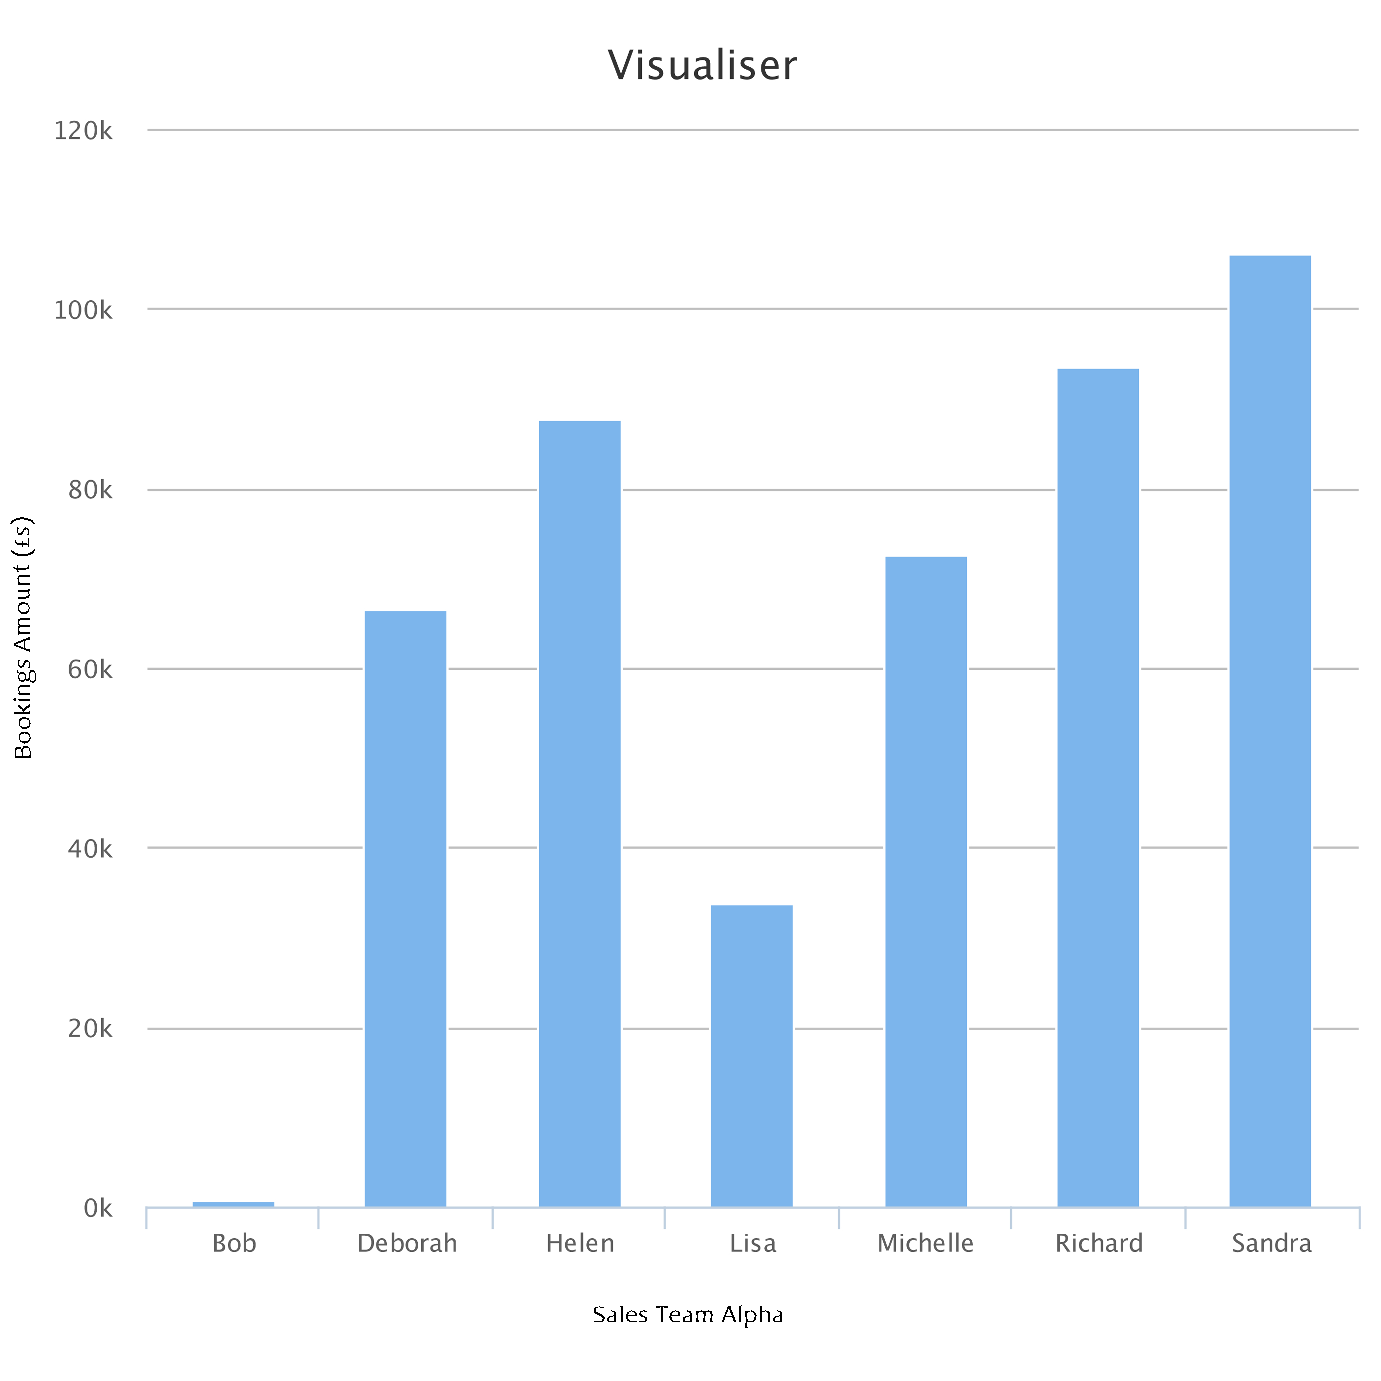
\includegraphics[scale=0.5]{chapter6/bar_chart}
\caption{Classic Bar Chart Data Visualisation}
\end{figure}

This chart is an easy and simple way to visualise the targets achieved by the employees against each individual name - and was used as the basis for a performance review. These are also helpful for drawing comparisons between employees and their performance, identifying trends in performance and combinations that produce better results within any organisation.

The more complex data visualisation are achieved through these simple form of representation with combination of more than one charts which helps in analysing data from different perspective. The data acquired from the previous layer, usually present data to the visualising engine in the form of an array. The array in listing 6 shows part of more complex data set.

\begin{listing}[ht]
\begin{minted}
[
frame=lines,
framesep=2mm,
baselinestretch=1.2,
bgcolor=LightGray,
fontsize=\footnotesize,
linenos
]
{python}


['Years',    'Web', 'Affiliates', 'In-Store',  'Door',  'Phone'],
['2008/09',   165,      938,       522,         998,     450],
['2009/10',   135,      1120,      599,         1268,    288],
['2010/11',    157,     1167,      587,         807,      397],
['2011/12',   139,      1110,      615,         968,      215],
['2012/13',    136,     691,       629,         1026,     366] ]);

\end{minted}
\caption{PAF Raw Data set Conversion Sample Code}
\end{listing}

The data is in an accessible form (extracted sample as above), this needs to be visualised. To do this a combination of tools including charts, API's, external Java Script visualisation systems and other pre-existing visualisation tools which are accessible to the system via the mashup application are utilised, the more complex examples such as transactional tagging and linked data visualisation codes are written for this research as the same output was not possible with the pre-existing technologies. \\

The concept behind the proposed research model is to represent complex data attributes in the simplest of visualised form. The visualised data is demonstrated in an area chart using one of the views and output systems in Figure 6.3. This visualisation practice can be considered as a non-coordinated, or single visualisation approach, and is commonly used within the field of information visualisation by various applications.\\

% Figure 6.3
\begin{figure}[H]
\centering
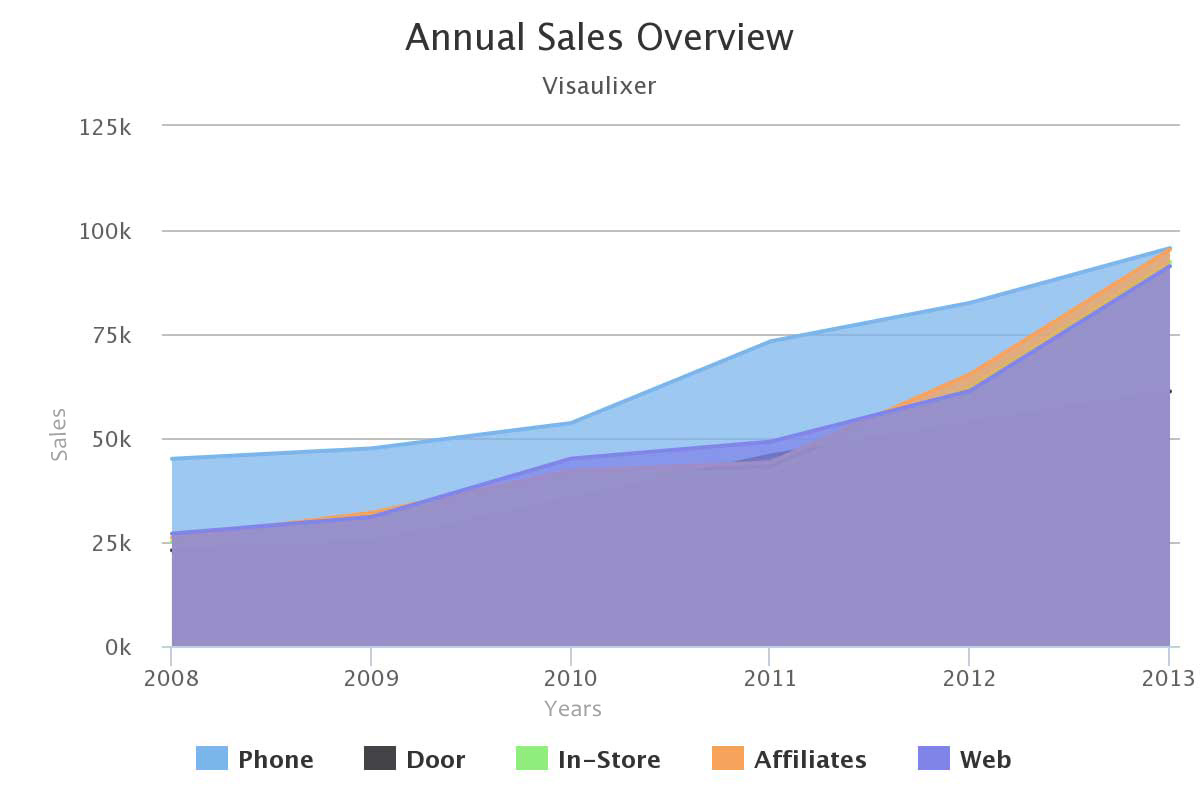
\includegraphics[scale=0.3]{chapter6/areachart}
\caption{Data Visualisation Through Area Graphs}
\end{figure}

This is just one visualisation layout, there are many different types available to end users, increasing the effectiveness of the interface layer and user interactivity, thus allowing it to function more smoothly. In the system there are many visualisation styles, all of which are available at the mashup application customisation layer, or through widget creation allowing users to create a section for each and every data set. 

This technique is often referred to as multi-coordinate visualisation, and is fast becoming the most popular and effective approach when decision makers need in depth information. This is because it is so flexible, versatile and fast; a business transaction picture can be drawn up from the data stored within the system in seconds, allowing decision makers to analyse data and cross examine various different aspects of the data in a single session. Figure 6.4 shows an example of a multi-coordinate visualisation. These simple data representation is interactive and provide more indepth analysis to users. Interactive graphs are not available in programs like Microsoft Excel. 

\begin{figure}[H]
\centering
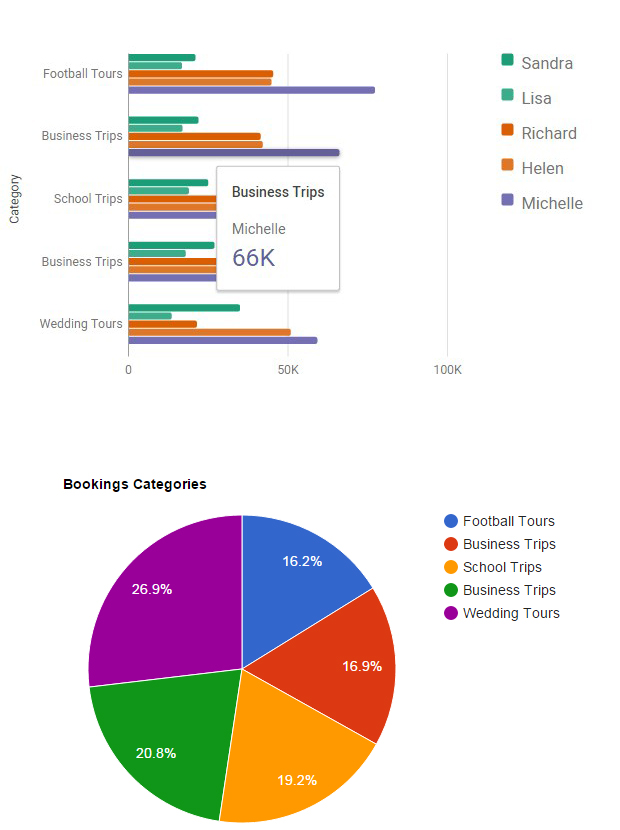
\includegraphics[scale=0.6]{chapter6/multicoordinatenew1}
\caption{Multi-coordinate Data Visualisation}
\end{figure}
%------------------------------------------------------
% Transactional Tagging Starts
%------------------------------------------------------

In information systems, tagging is considered non-hierarchical terms assigned to a particular action or sub data elements. Tags are usually added to digital media such as images, videos, audios or computer files. Tags are also very popular in social media websites such as Facebook. It is also some time known as folksonomy \cite{o2009web}. However, it is popularised with the introduction of user generated content in Web 2.0. Tagging helps with data classification and categorisation. Similar approach for the acquisition and data analysis layer in the visualisation model proposed in this research. Its a novel contribution to data analysis field specially to transactional data. The web intelligent explore relations between data elements and the repositories are then retrieved for the data representation layer. The end user at the enterprise environment is also given the ability to tag information. Thus a two-way tagging approach adapted by the system which helps in validating transactions before any analysis is done. Transactional tagging also helps in visualising multiple dimensional data as many attributes could be explored within one visual graph. Figure 6.5 shows an image extracted from the system visualising sample data from the transactional data set.\\
% Figure 6.5
\begin{figure}[H]
\centering
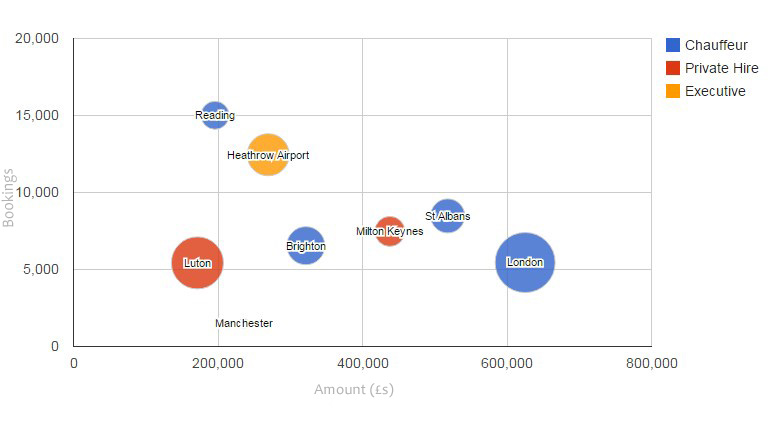
\includegraphics[scale=0.5]{chapter6/Linked_data/transactional1}
\caption{Transactional Data Tagging Visualisation}
\end{figure}

The data which has been visualised is from the bookings table in the transactional data set used in this experiment. Multi-coordinate visualisation has the ability to visualise diverse data and helping users in exploring data trends. For example, in Figure 6.6 various bookings types are highlighted including transactions channels such as web sales, email sales, BDM (Business Development) and phone sales. The same data is further visualised showing which resources (vehicles) were allocated to different categories. Kelly and Klassy were used with orders taken over the phone. Dympa, Becky and Valarie vehicles were used for orders taken through web channels. This kind of data analysis helps decision makers to optimise resource management and revenue streams.

\begin{figure}[H]
\centering
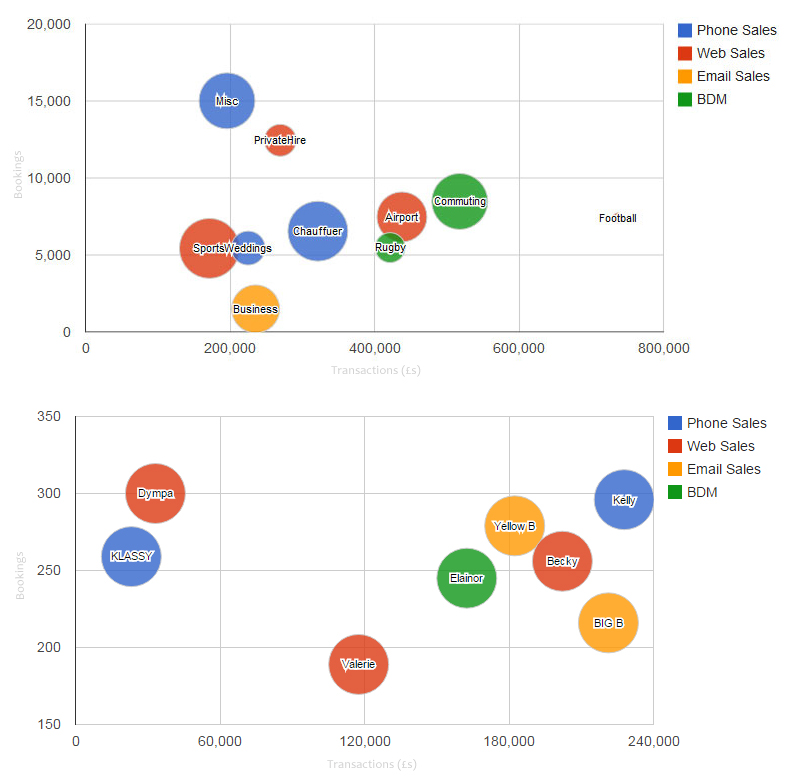
\includegraphics[scale=0.5]{chapter6/Linked_data/multi-tagging}
\caption{Tagged Bookings in Multi-coordinate Visualisation}
\end{figure}

Figure 6.6 demonstrates tagged data in multi-coordinate visualisation form - making it very easy for the end user to cross examine information. The same principle could be applied to any data where multi-attribute data visualised for more in depth analysis and insights.

%-------------------------------------
% Transactional Tagging Ends
%--------------------------------------

%------------------------------------
% Link Data Starts 
%------------------------------------

The Semantic Web is the combination of different types of data elements combined together forming semitic data — the data could be elements of online orders, bookings, articles, financial data, governmental data and available in so many other forms and formats. However, for the linked data phenomenon, it is very critical to have the huge amount of data on the Web available in a standard format, accessible and retrievable by the web tools and applications \cite{bizer2009linked}. The same concept could be applied to transactional data sets or any other data set available to computer systems for analysis purposes. The data should be transformed or made available in a semantic or a standard format where data relations are explored and discovered. The linked data approach has been adapted to find relations and furthermore, visualise those relationship making it easy for the users to analyse complex data sets. An identical approach as that to linked data is applied to different data sets and then the data relations are visualised as a sub set of the main visualisation problem. The following examples will highlight the technique and usage of the linked data visualisation.

% Figure 6.7
\begin{figure}
\centering
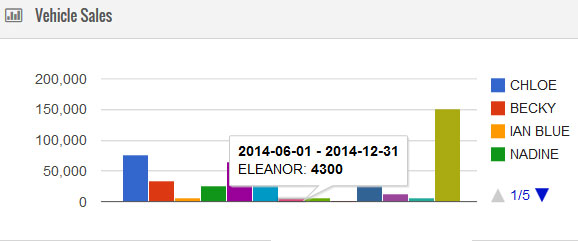
\includegraphics[scale=0.6]{chapter6/Linked_data/vehicles}
\caption{Bar Chart for Linked Data Visualisation}
\end{figure}

The visualisation process is taken place at the same time with other elements of data set. For this exercise, data from the commercial data set has been used. The extracted data shows vehicle sales values in Figure 6.7 for a specified date range. The bar shows each vehicle sales values, upon clicking on a vehicle bar, the locations of the sales are highlighted on an interactive map for the selected vehicle as shown in Figure 8. At the same time, another multi-coordinate chart is generated and showing tagged bookings for the same selected vehicle.

\begin{figure}
\centering
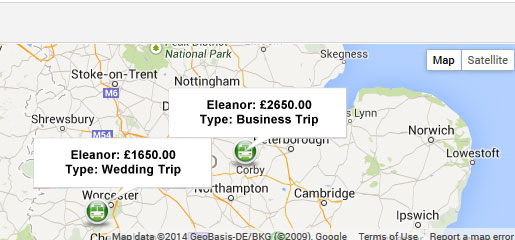
\includegraphics[scale=0.8]{chapter6/Linked_data/geo}
\caption{Live Map for Linked Data Visualisation}
\end{figure}

% Figure 6.9
\begin{figure}
\centering
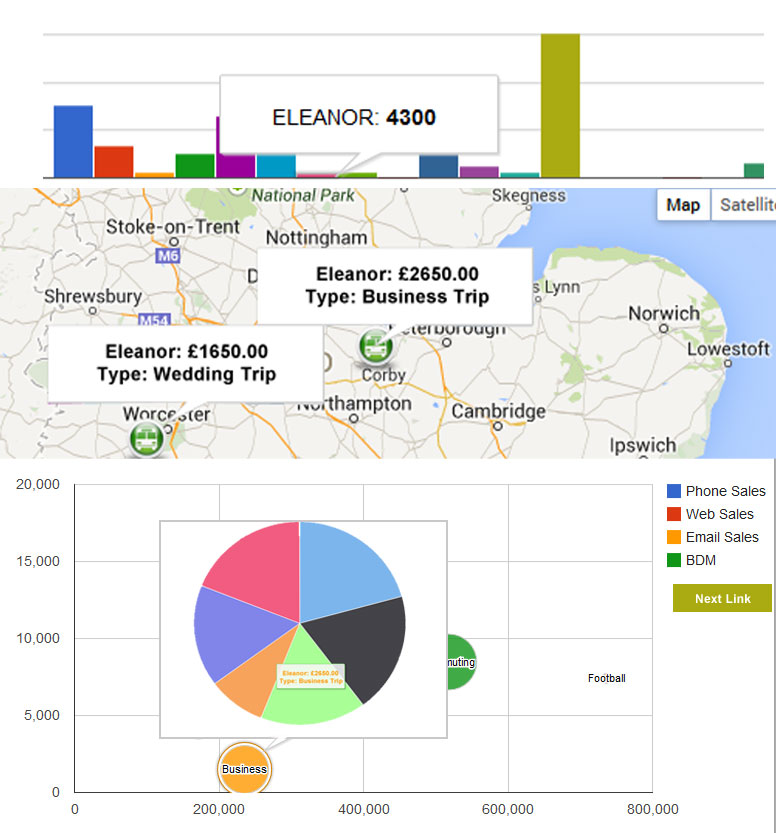
\includegraphics[scale=0.47]{chapter6/Linked_data/part1}
\caption{Multi-attribute and Multi-Coordinate Linked Data Visualisation}
\end{figure}

Figure 6.9 highlights, data element relation in a visualised form. The first part in the image shows some of the vehicles and while clicking on a particular vehicle, in this instance Eleanor, shows two additional charts. The second chart shows information about booking location on a live and interactive map. The third chart shows tagged bookings medium and industry related to this particular vehicle. If the tagged medium and industry are more than one, more information is shown on clicking on the next button, which then produces visualisation of next related data elements as illustrated in Figure 6.10.

\begin{figure}
\centering
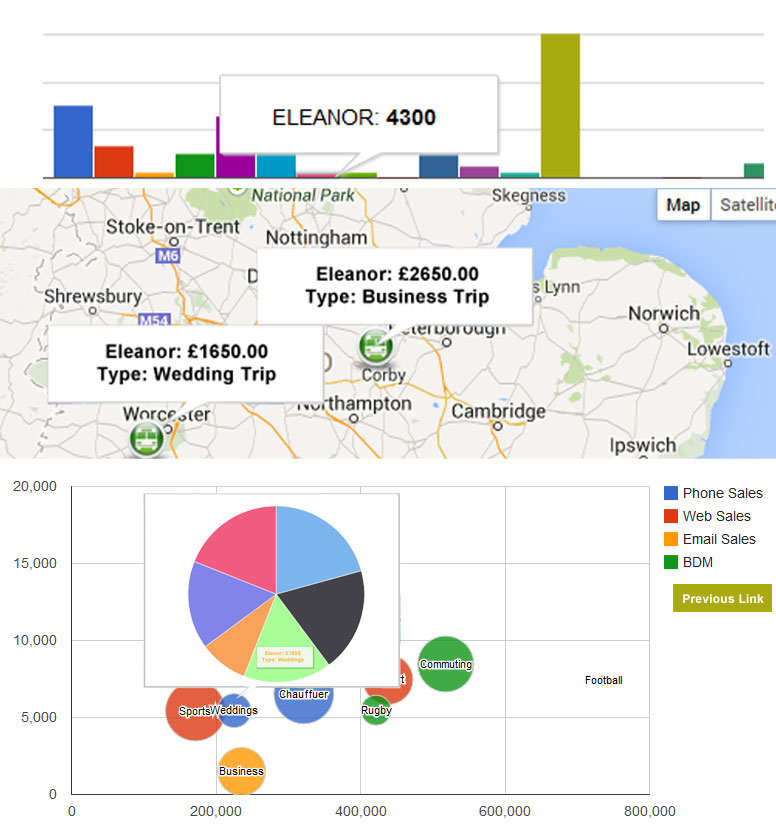
\includegraphics[scale=0.5]{chapter6/Linked_data/part2}
\caption{More Insights Based Linked Data Visualisation}
\end{figure}

The linked data visualisation is a novel contribution in information visualisation. The model first explores relationships within the data sets as demonstrated above and then visualise the information for end user providing ease of understanding and decision making on a particular asset or resource. The linked data visualisation concept is further discussed in the next chapter with a different set of experiment and data types.

%---------------------------------
% Linked Data Ends
%---------------------------------
The Visaulixer tool, designed and developed for the information visualisation model will come into action where data sets are not in normalised or structural form, in other words data sets are in non-enterprise environment. The data import features of the system are explained in the previous acquisition and data analysis section in this chapter. There are various examples of graphs generated by the Visualixer tool at the data representation layer. In the next section, the system interaction features will be highlighted and discussed for business transactional data sets.

\section{Interactivity}

The two important aspect of the system are discussed, as how users interact with the application and the application interaction with the data and the data representation layer. The fundamental aspect is accepting input from a user. Interactive computer systems are functions and programs which allow users to enter data or instruction to the application through interfaces. The applications respond to user requests through these interfaces by providing what the users want to see or expect from the system. Computer programs or devices (in response to a user's action or request) presents choices (paths) depending on where in the program the user has initiated the action. Using these choices, the user can control or change the action of the device or outcome of a game or program. Interactivity is key element in the proposed information visualisation system. The users are given option to interact with visualised content. Furthermore, ability to export information at the interact++ layer. 

In the proposed system, the user has the unique ability to tweak the input or change the data questions, and the system, the intelligent design enable it to accept the changes easily (no matter how challenging) and alter the outcomes, producing output based on the users instructions. All of these various outputs are in the form of interactive charts and graphs of data, which are quickly processed by the proposed system without any problems. With the addition of interactive graphs into the mix, application is able to give additional information which is not always available or visible on the static graphs produced, but nonetheless connected or associated with an event. With interactive graphs, such events are just a mouse click (or hover) away and these graphs will generate more data and information for the analysis purposes. The interactive aspect of the system are utilised in Figure 6.11, the user is given an option to click on area of interest to explore more in-depth information.\\ 

% Figure 6.11
\begin{figure}[H]
\centering
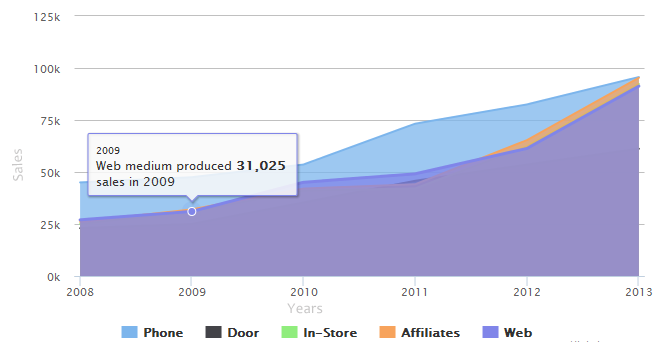
\includegraphics[scale=0.6]{chapter6/mouseover}
\caption{Graph Interaction on Hover}
\end{figure}

These new graphs have another unique ability, it can be used to drill down further into the data; revealing more detailed analysis and allowing us to view non-aggregated visualised information. The interactive layer also allows to zoom-in and zoom out on specific features available in various graphs, and this just adds to the power of this new technology. The interactivity of the graphs is a key feature in helping to achieve a much greater and deeper understanding of the most complex data elements, without the headache of manual analysis. The user have been given the ability to pick and choose different types of data for further analysis, if the user want to see or compare phone orders, it could be achieved with only disabling rest of the elements of the graph as illustrated in Figure 6.12.

%Figure 6.12
\begin{figure}[H]
\centering
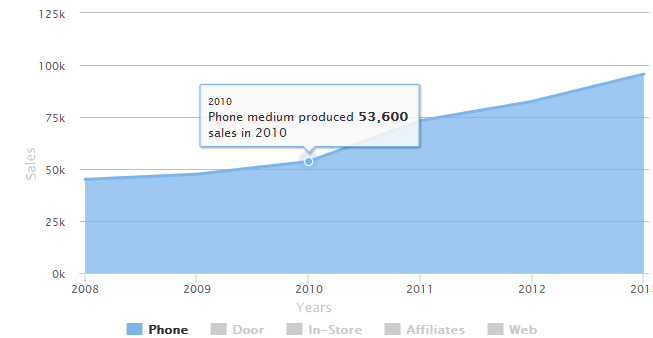
\includegraphics[scale=0.6]{chapter6/mouseover2}
\caption{Selection Option for In-depth Analysis}
\end{figure}

In addition to all of the above, there are also extras that can be added to the interactive graphs to improve their effectiveness and reveal yet more information for comprehensive analysis. There are various data filters which can be applied to the interact++ layer, and these filters have various functions within the layer. The data set has been visualised in its totality. For example, if a system has visualised the booking information for the period of a single month, this could be filtered into a date range that spans two months, depending on the date range used, or even reduced to one day.  The filters can be applied to understand the data more clearly, or to answer a particular data question the user might have. For example, a member of management might want to know how many bookings the sales team have taken in a week, a month or in a single day as in Figure 6.13.

% Figure 6.13
\begin{figure}[H]
\centering
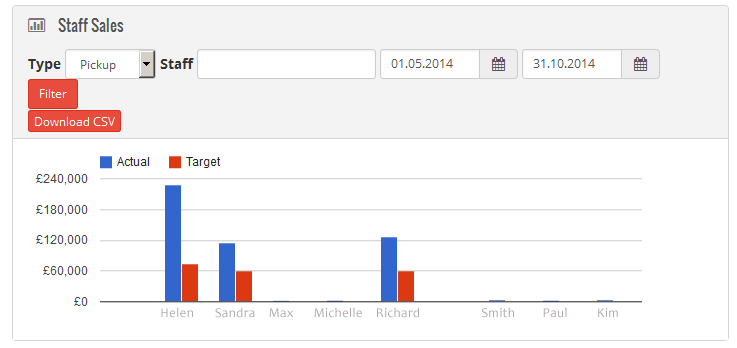
\includegraphics[scale=0.5]{chapter6/salesfiguresdaterange}
\caption{Data Analysis at Interact++ Layer}
\end{figure}

There are filters that can be applied to help the user to determine where this information lies, access it and bring it forward. The filters applied could also be more unique in nature, applied to unique data elements, for example to filter by staff members. This would help answer the query, how many bookings did staff member X generate in one week, or one month? These unique and incredibly useful interactive filters are simply instructions by the users, to display or retrieve information that users have shown an interest in. Interactive presentation is now the focal point of the proposed system, as this technique leads to deeper knowledge and understanding, as well as unearthing hidden trends and patterns about the data sets.

\section{History}

Data graphs which have been generated at the interactive layer also have an extra feature where data can be exported into a specific format such as PDF, JPEG, GIF or even other types of charts and graphs when requested. The history layer within the program allows the user to store generated graphs and charts, and make them accessible to other users upon request. This history element is particularly effective for the comparison or charts and graphs at a later stage; perhaps to review progress or look back on statistics to make judgements on new business strategies.

\section{Summary}

In this chapter, the visualisation model was tested with huge business transactional data set. The enterprise and non-enterprise scenarios are discussed based on how data is acquired and analysed in both of these environments. The data sets where data was not in normalised source, Visualixer data analysis model was presented to support the visualisation process. The data representation layer was then supported with various graphs and charts generated by the system. The user interaction with the system explained and evidence provided with screen shots from the application. The system ability to store information in various formats are discussed in the final section of the chapter. 

Linked data visualisation is introduced and tested with transactional data set. The transactional tagging also explained with the same data set. Multi-attribute and multi-coordinate visualisation techniques are demonstrated with various charts in this chapter. In the next chapter, further discussion of the two experiments is undertaken. The visualisation model and its outcomes are compared with existing tools and technologies.